\documentclass[a4paper,12pt]{article}
\usepackage[francais]{babel}
\usepackage[T1]{fontenc}
\usepackage[utf8]{inputenc}
\usepackage{pslatex}
\usepackage{url}
\usepackage{graphicx}
\usepackage{lscape}
\selectlanguage{francais}


\title{Rapport de Soutenance 2}
\author{
Ihy Group : \\
deguil\_x (Xavier Deguillard)\\
genite\_n (Nicolas Geniteau)\\
sezer\_s (Stephane Sezer)\\
wagnac\_t (Teddy Wagnac)
}

\begin{document}

\maketitle

\newpage

\section*{Introduction}

\newpage

\tableofcontents

\newpage

\section{Travail accompli}
	\subsection{Lecture du format}
Un pré requis la création d'un codec est sa lecture, le format doit
pouvoir être lu tel quel, et non pas décompressé vers un fichier wav pour
pouvoir ensuite le lire, on
perdrait alors tous intérêt d'un tel format. Il faut donc mettre en place un
système de ``streaming'' dans lequel la décompression et la lecture sont
simultanés.
		\subsubsection{Architecture du streaming}
La première idée qui vient à l'esprit, est d'attendre qu'une partie de la
musique soit lue pour commencer à décompresser puis lire ce que l'on vient de
décompresser. Malheureusement, cette implantation naïve ne fonctionne tout
simplement pas. En effet, décompresser un ``chunk'', c'est-à-dire un bout de la
musique, n'est pas une opération instantané, et donc par conséquent, la lecture
aurait marqué un temps d'arrêt à la fin de chaque chunk, correspondant à la
durée de décompression dudit chunk.\\
Pour pallier à ce problème il faut threader la décompression, à l'aide de deux
processus séparés. Le premier processus va décompresser les chunks pendant que
le second va lire les chunks que le premier processus aura décompresser. Comme
la décompression dure moins longtemps que la lecture, il n'y a pas de temps
d'arrêt notable lors d'un changement de chunk.\\
Pour mettre en place cette solution, il nous a fallu penser de façon parallèle,
en effet si la programmation séquentielle va de soit, il n'en est pas de même
pour la programmation parallèle. Et la se pose le premier problème, comment
communiquer entre ces deux processus?\\
		\subsubsection{Le buffer}
Ce qui ici est essentiel, est une structure de données partagées entre les
deux processus. Pour cela, un buffer est
tout approprié. En effet, lorsque le processus de lecture a besoin de données
décompressées, il va simplement récupérer le prochain élément du buffer, et
lorsque le processus de décompression a fini de décompresser, il va tout
simplement ajouter les données dans le buffer. On voit ici clairement qu'un
buffer n'est qu'une simple structure de donnée de type ``fifo''\footnote{first
in first out}, qui est souvent implanté avec une file.\\
Notre buffer est néanmoins plus complexe qu'une simple file, en effet, il faut
qu'il puisse gérer les accès concurrentiels de la part des deux processus. Pour
cela, on utilise des ``mutex'' pour protéger les zones critiques, plus
précisément, l'ajout et le retrait d'un élément. De plus, pour des raisons
d'économies de mémoire et d'activité du processeur, il est judicieux que le
processus de décompression ne
soit pas toujours actif, en effet, lorsqu'un chunk est décompressé, il contient
uniquement des échantillons, tels qu'ils sont codés dans un fichier wav, tout
décompresser en une seule fois reviendrai a avoir le fichier wav intégralement
en mémoire. En plus de cela, la lecture audio de notre format ne doit pas
impacter les performances de l'ordinateur. Pour régler ces deux soucis, il
existe une solution plutôt simple, définir une taille maximum pour le buffer, et
lorsque celui-ci est plein, le processus de décompression va tout simplement
attendre que ce dernier se vide. La ``bonne taille'' a été déterminée et est une
taille de buffer de trois, c'est-à-dire que le buffer ne peut contenir que
trois chunks.\\
		\subsubsection{Sortie audio}
Lorsque tout ceci fut mis en place, il ne restait plus qu'à utiliser ce que nous
avions commencé à mettre en place à la soutenance dernière, en prévision de
cette lecture en streaming, la lecture d'un fichier wav. Ici, lorsque l'on
décompresse le ihy, on récupère des bouts de wav, qui correspondent aux chunks
du format. Il ne reste alors plus qu'à les envoyer à libao, pour que ce dernier
nous le lise.
	\subsection{Le type half}
	\subsection{Ondelettes}
A la soutenance precedente, nous avions implemente l'ondelette de
haar. Il s'agit de l'ondelette la plus simple a mettre en oeuvre mais
n'est pas la plus adapte pour la compression d'un signal audio.
Nous avons donc voulu en tester une autre. De nombreuses recherches
nous ont appris que la famille d'ondelette de Daubechies donnaient en
general de bons resultats mais que cela pouvait varier en fonction du
signal a compresser.\\
\subsubsection{Ondelettes de Daubechies}
Les ondelettes de Daubechies est une famille d'ondelettes respectants
certaines proprietes bien precises. Il s'agit de l'ondelette ayant le
plus petit support compact pour un nombre choisi de moments nuls. Pour
p moments nuls, le support de l'ondelette correspondante est de 2p. En
effet, il a ete demontre par Ingrid Daubechies que toute ondellette a
p moments nuls a au moins 2p coefficients non nuls. Or les ondelettes
de Daubechies en ont exactement 2p. On peut donc dire qu'elles est
optimal en ce qui concerne les moments nuls.\\
Il existe donc une infinite d'ondelettes de cette famille qui sont
caracterise par le nombre de moment nul. Haar est par exemple une
ondelette de Daubechies avec un moment nul. Il reste donc plus qu'a
implementer cette ondelette pour un p quelconque.
\subsubsection{Implementation des ondellettes de Daubechies}
L'implementation de ces ondelettes nous ont cause de nombreux
problemes que nous n'avions pas prevus.\\
Premierement, la comprehension mathematique de cet outil n'a pas ete
facile car il nous manquait encore des bases (tel que les Series de
Fourriers que nous voyons que maintenant). Heuresement notre
professeur de mathematiques nous a conseille un excelent livre sur les
ondelettes de Stephane Mallat qui nous a permis de combler certaines
de nos lacunes. Une fois que nous avions compris les differents
theoremes, il fallait encore les transformer en algorithmes utilisable
dans notre projet. Ca a ete plus dur que ce que nous pensions.\\
La, nous avons rencontre un nouveau probleme auquel nous n'avions pas
pense : les coefficients de bords. En effet, les ondelletes est un
principe mathematique qui s'applique sur un signal infini. Or dans
notre cas, le signal a bien evidement un debut et une
fin. Concretement, pour la transformee par ondelette, on a besoin des
valeurs precedentes pour les premieres valeurs et les suivantes pour
les dernieres valeurs alors qu'elles n'existent pas. Il existe 3
methodes pour pallier ces effets de bords. La premiere consiste a
rendre le signal periodique et de le rendre cyclique. C'est assez
simple de le mettre en place mais cela entraine de grands coefficents
aux extremites et n'ont plus reelement de sens physique. Ce n'est donc
pas adapte pour la compression du signal.\\
Une deuxieme solution existe mais uniquement sur les ondelettes
symetrique or il a ete prouve que Haar est la seule a l'etre. Or Haar
n'a pas ce probleme d'effet de bord car son support est de seulement
2.\\
Nous avons adopte une autre methode qui consiste a utiliser des
ondelettes de bords adaptees, ayant le meme nombre de moments nuls
afin d'eviter de grands coefficients de bords. Cette methode est celle
qui donne les meilleurs resultats mais est aussi la plus dur a mettre
en oeuvre. Nous avons eu beaucoup de mal a cause du manque
d'informations sur cette technique.\\
Nous avons rencontre un dernier probleme algorithmique. En effet, la
formule general de la transforme par ondelette a une complexite bien
trop eleve (on arrivait a plusieurs heures pour la compression de
quelques minutes de musique). Nous avons donc du optimise
l'algorithme, comme nous l'avions fait pour Haar, en fonction de
p.\\\\
Ces nombreux soucis nous ont donc quelque peu ralenti dans notre
avancee et pour le moment seul la compression avec l'ondelette de
Daubechies marche correctement. Il restera donc encore a faire la
decompression pour la prochaine soutenance.
\subsection{Traitements des coefficients}
Une fois la transformee par ondelette effectue, nous recuperons un
grand nombres de coefficients qu'il faut encore traiter pour avoir une
bonne compression avec huffman. Pour que ce soit efficace, il faut
avoir un maximum de valeurs identiques. Pour cela, nous appliquons
pour le moments trois filtres differents.
\subsubsection{Suppression des coefficients de petites echelles}
La premiere etape et de supprimer les coefficients correspondants aux
petites echelles. En effet ceux-ci influent globalement sur les hautes
frequences qui ne sont pas percu par l'oreille humaine. On peut donc
deja supprimer la moitier des coefficients.
\subsubsection{Suppression des coefficients proches de zero}
La deuxieme etape est de supprimer tout les coefficients relativement
prochent de zero. La encore ces coefficients agissent que tres peu sur
le signal final. Il a donc fallut trouver une valeur limite pour
laquel on pouvait considerer que coefficients en dessous de cette
valeur etait negligeable pour l'oreille.
\subsubsection{Egalisation}
La derniere etape est l'egalisation des valeurs. En effet Huffman est
efficace si on a de nombreuses valeurs similaires. On parcourt donc le
tableau de coefficients en recherchant les valeurs qui sont
relativement proches puis on les remplacent par la valeur
moyenne. Encore une fois, il a fallut trouver cette limite.
	\subsection{Threading}
	\subsection{Huffman suite et fin}
À la dernière soutenance, nous pouvions utiliser huffman, pour compresser des
données, néanmoins, nous n'avions pas écrit le code pour la décompression, et
donc nous ne pouvions pas savoir si cela marchait réellement, nous savions juste
que cela devrait marcher théoriquement. Nous avons donc écrit le code pour
décompresser Huffman, et bien sûr, cela n'a pas fonctionné dès le début (ça
aurait été trop beau). En fait, la technique utilisée à la compression, pour
l'écriture était mauvaise, après réécriture de cette partie du code, tout
marchait.\\
La technique utilisée pour décompresser des données qui ont été précédemment
compressées via Huffman est simple, on récupère le prochain bit des données
compressées, puis si il s'agit d'un 0, on recommence le procédé sur le fils
gauche de l'arbre, si c'est un 1, à droite. Enfin le caractère non compressé est
celui que l'on trouve lorsque l'on arrive en racine de l'arbre de Huffman, que
l'on avait, à la compression, sauvé dans le fichier. Pour décompresser
totalement le fichier, on recommence ce petit
procédé tant qu'il y a des caractères dans celui-ci.\\
Contrairement à notre première idée, Huffman n'est pas appliqué sur tout le
fichier, il n'y a pas un arbre unique pour tout le fichier. En fait, chaque
chunk possède son propre arbre de Huffman, cela permet d'avoir un arbre de
Huffman qui est beaucoup plus précis et donc, de gagner en compression, en
contrepartie, l'arbre de
Huffman doit être écrit pour chaque chunk. Il fallait donc trouver le bon
compromis, afin d'avoir une compression optimale. À cause des ondelettes, la
taille d'un chunk doit être une puissance de deux, les tests pour l'optimalité
de Huffman ont donc été assez facile à réaliser. Sans avoir fait de tests (et
même avant d'avoir commencer Huffman), nous avions fixé la taille d'un chunk
comme étant équivalente à 65536 échantillons, et coup de chance pour nous, il
s'agit de la taille optimale pour Huffman, un chunk deux fois plus gros, ou deux
fois plus petit, grossis la taille du fichier final de quelques
kilo-octets.\\

\newpage

	\subsection{Interface graphique}
À la première soutenance, nous avions une interface graphique basique avec une 
barre de progression et les boutons standard d'un lecteur audio. Cette dernière 
nous a permis de nous familiariser avec cet outil qui n'est rien d'autre que 
GTK+. Maitenant, pour cette soutenance, notre interface à quelque peu évoluée grâce 
notamment à l'intégration de cairo dans notre projet...
	\subsubsection{La structure de l'interface}
Dans notre premiere ébauche d'interface, nous utilisions des box pour placer les
différents widgets dans la fenêtre. Mais ce n'est pas la meilleure solution si 
on veut placer ses widgets à des endroits précis. Donc nous avons tout simplement 
décidé d'utiliser une Table de 9 lignes et 9 colonnes. En effet, c'est un container 
de GTK+ qui utilise une grille invisible pour attacher les widgets. Donc il suffit 
d'intégrer les widgets dans la table et de les positionner grâce à des coordonnés.
Ce qui est plus avantageux qu'une Box qui elle positionne les widgets quasiment 
alléatoirement. Grâce à cette table, notre interface détient une barre de progression 
et les boutons standard d'un lecteur audio comme à la première soutenance, mais aussi 
une barre de menu et une zone de dessin (nous y reviendrons plus tard). Pour les boutons, 
nous avons tout de même utilisé une Box pour les contenirs avec une dimension précise et un 
espace entre eux nul. Comme pour la dernière soutenance, la jauge se remplit quand
le bouton "Play" est activé, avec le même principe que la dernière fois. De plus, nous avons une 
barre de menu qui ne contient pour le moment que l'option "File". Dedans, on peut y trouver les boutons
"New" qui servira certainement à créer une nouvelle playlist, "Open" qui lui servira à 
récupérer un fichier de format Ihy dans son disque afin de pouvoir l'ouvrir et enfin 
le bouton "Quit" qui permet tout simplement de fermer l'application.
	\subsubsection{La zone de dessin}
Pour cette soutenance, nous devions intégrer dans notre interface une zone afin
d'entamer le spectrographe. Pour se faire, nous avons décidé d'utilisé Cairo.
Cairo est une bibliothèque logicielle graphique libre qui définit une API de
rendu vectoriel 2D indépendante du matériel. De plus, cairo est parfaitement
utilisable avec GTK+. Nous avons donc aujourd'hui, une zone de dessin de
dimension 500x500, en fond noir, avec pour le moment dedans, deux étoiles en
mouvement. La première étoile, réalise un mouvement de translation et rotatif 
grâce aux fonctions cairo-translate() et cairo-rotate() toute deux issues de la
bibliothèque de cairo. Tandis que la seconde étoile, elle, réalise un
mouvement de translation et rotatif mais aussi un mouvement d'échelle qui
provoque une impression de va et vien de l'étoile dans la zone de dessin. Ce
mouvemente est réalisé grâce à la fonction cairo-scale.\\
Cependant, cette petite zone de dessin nous a posé problème pour l'intégration dans
notre interface. En effet, la fonction qui permet de créé la zone de dessin avec
les bibliothèques de cairo ne crée pas un widget directement. Ce qui est quelque
peut embétant car la fonction qui permet d'intégré quelque chose dans une table
n'accepte que les widgets. Par conséquent , nous décidons de créer un GdkPixmap
qui contiendra la zone de dessin et qui sera détenue dans un widget grâce à la
fonction gtk-pixmap-new().  
	\subsubsection{Pour la prochaine fois...}
Donc, pour la dernière soutenance, nous espérons terminer l'interface avec
l'intégration d'une playlist, de la fonction qui dessine dans la zone de
dessin en fonction de la musique, et en activant quelques widgets en plus. Pour
le moment, voici notre interface actuel 
\begin{center}
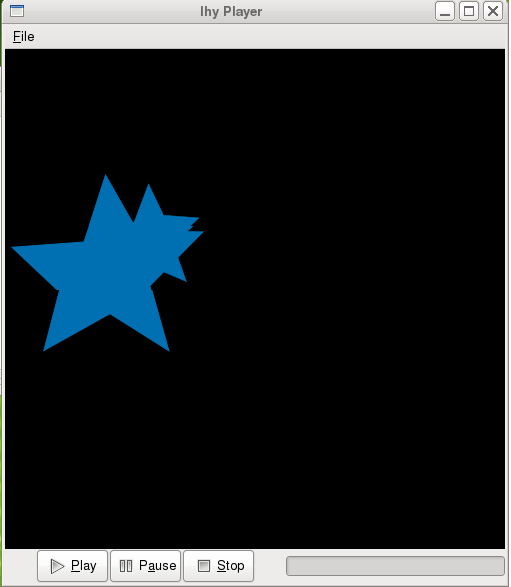
\includegraphics[scale=0.50]{Player.png}
\end{center}

\newpage

	\subsection{Portage sur iPhone}
Aujourd'hui, les codecs audio sont de plus en plus utilisés sur des
ordinateur possédant une puissance plus que limite, j'ai nommé les iPods
et dérives. Pour qu'un codec soit considère comme utilisable, il faut
qu'il puisse être utilise sur ces plateformes, cela montre qu'il n'est
pas nécessaire d'avoir un ordinateur très puissant pour pouvoir lire le
format. C'est également une preuve d'un codec bien réalise, celui ci
étant alors portable et donc théoriquement lisible sur tous les
appareils.\\
L'année dernière apple a sorti un SDK\footnote{software developpement
kit} permettant de développer des applications pour l'iPhone\footnote{Lorsque
l'on parle d'iPhone, on parle également d'iPod Touch, qui sont identiques au
niveau plateforme de développement}, ceci en
utilisant les outils ainsi que la documentation officielle, et ce de façon gratuite.
C'est l'occasion rêvée de montrer que notre codec est a la fois
portable et léger.\\
		\subsubsection{Reunir les outils}
Première étape donc, absolument indispensable a la réalisation du
portage, la mise en place d'un environnement de cross-compilation,
c'est-à-dire, un compilateur, et les outils associés,  pouvant générer du code
pour iPhone, qui
tourne sur un ordinateur classique. Le SDK de apple en fournit un, mais
celui-ci est compatible uniquement avec MAC OSX Leopard, ce que nous ne
possédons pas. Heureusement, la communauté ``underground'' de l'iPhone
est assez importante, en cherchant bien, on a réussi a trouver un
tutoriel expliquant comment se construire un
``toolchain''\footnote{logiciel et headers complet pour compiler un
programme} intégral sur Linux. Après cela, nous pouvions compiler et lancer un
simple Hello World sur l'iPhone.\\
Mais voila, notre projet n'est pas uniquement fait de C, mais également
de OCaml. Il a donc fallu trouver une façon de créer un compilateur
cross-compilateur OCaml
pour l'iPhone. On a également trouvé un tutoriel très détaillé, fournissant les
patchs a appliquer aux sources de OCaml, pour que celui-ci génère du code pour
iPhone.
		\subsubsection{Compiler le projet}
Notre projet ne possédant que très peu de dépendance externes, la
compilation s'est bien déroulée, sauf sur la seule dépendance : libao, la
bibliothèque nous permettant de lire du son. Après l'avoir retire du
projet, nous avons teste le bon fonctionnement des autres composants du
projet, c'est-à-dire la compression et la décompression. Cela a
fonctionné du premier coup, chose a laquelle je ne m'attendais pas.\\
		\subsubsection{La sortie audio}
Libao ne compilant pas, il nous fallait impérativement trouver une autre
solution pour lire du son. En fouillant dans la documentation de Apple, je suis
tombé sur un article montrant comment utiliser les ``Audio Queues'', qui est
décrit comme étant ``la solution pour lire vos sons de façon asynchrone''. La
description colle exactement avec l'utilisation qu'on veut en avoir.\\
Dans les grandes lignes, apple a implanté la notion décrite plus haut pour
les buffers audio, et l'a rendue utilisable via ces Audio Queues. La seule chose
à faire est de créer une fonction qui sera appelée lorsque le lecteur audio aura
besoin de nouvelles données. Dans notre cas, cette fonction va tout simplement
décompresser le fichier ihy et le renvoyer sous la forme d'un flux PCM.\\
Lorsque cela fut implanter, l'iPhone pouvait lire, de façon théorique, notre
format. Restait à le vérifier sur l'iPhone. Et là oh surprise, cela
fonctionnait, de façon totalement fluide. 
	\subsection{Site web}
Ce dernier n'a pas beaucoup évolué, au niveau de l'interface depuis la dernière
soutenance. Néanmoins, des changements non visible ont été fait. En effet, à la
dernière soutenance, le site n'était absolument pas valide avec la norme w3c, et
présentait un total de 19 erreurs, cela faisait beaucoup pour une seule
page\ldots\\
De plus, des news ont été ajoutées, pour que les internautes puissent connaître,
sans à avoir à regarder le code et les messages déposés sur le git, l'avancement
du projet, les nouvelles fonctionnalités, ainsi que les futures. Une news fait
même office de tutoriel pour compiler et utiliser le codec ihy sur un iphone
(voir ci-dessus), cette dernière expliquant très précisément les différentes
étapes à suivre pour que tout fonctionne.

\newpage

\section{Tâches prévues}
	\subsection{Documentation}
Pour cette ultime soutenance, nous avons prévu d'écrire une documentation du
format, suffisamment détaillée pour que n'importe qui puisse lire et écrire un
fichier ihy sans dépendre de notre code. Il s'agit d'un pré requis pour
l'utilisation de n'importe quel codec. Seul les firmes multinationales
maîtrisant à la fois le système d'exploitation et les logiciels, peut se
permettre de ne pas donner les spécifications d'un codec.\\
Cette documentation contiendra plusieurs choses. Premièrement, la description
complète des ``headers'' du format, ces derniers étant indispensable à la
décompression du fichier. Deuxièmement, une description des algorithmes
utilisés, ou pouvant être utilisés. Et enfin, l'ordonnancement des données dans
le fichier compressé, comme par exemple, la façon dont l'arbre de Huffman est
stocké.
	\subsection{Comparaison entre les codecs}
Un élément indispensable lors de la finalisation d'un codec audio (ou vidéo),
est sa comparaison avec les codecs existants. En effet, un nouveau codec ne
faisant rien de nouveau, compressant moins bien, ou ayant une qualité à l'écoute
moins bonne a peu de chances d'être utilisé.\\
Il faudra donc, montrer les points forts de notre codecs fasse aux concurents
que sont par exemple le mp3, ogg, wma, etc. Tout en essayant de masquer au
maximum les points faible de notre codec\footnote{Cette partie aurait pu être
nommée ``Publicité''}.\\
Les points comparés seront donc, la qualité d'écoute, un facteur extrêmement
objectif, ne pouvant être chiffré, la taille du fichier final, le spectre audio,
qui devrai confirmer les résultats du premier test, et enfin, la rapidité de
compression et de décompression, ainsi que la charge CPU lors de la lecture d'un
fichier.

\newpage

\section*{Conclusion}

\end{document}
